\section{Observations and Calculations}

    \subsection{Observational Data}
    \begin{itemize}
        \item Least count of the micrometer = 0.01mm
        \item Breadth of the glass slab ($b$) = 49.4mm
        \item Depth of the glass slab ($d$) = 2.07mm
        \item Distance from the knife-edge to the load ($l$) = 115mm
    \end{itemize}
    
    \subsubsection{For $\text{m}_1$ = 200g}
        \begin{table}[H]
    \centering
    \begin{tabular}{|c|c|c|c|c|c|}
        \hline
        Fringe    & Fringes on     & Fringes on       & $\text{D}_x$        & $\rho_x$   & $\text{R}_x$    \\ 
        Order     & the left (mm)  & the right (mm)   & (mm)       & ($\text{mm}^2$)   & (mm)   \\ \hline
        1 &  9.24 & 5.40 &  3.84 &     &     \\
         2 & 10.38 & 3.89 &  6.49 &  6.84 & 11.62 \\
         3 & 11.18 & 3.02 &  8.16 & 12.96 & 11.00  \\
         4 & 12.41 & 2.23 & 10.18 & 22.22 & 12.58 \\
         5 & 13.05 & 1.48 & 11.57 & 29.78 & 12.64 \\
         6 & 13.55 & 0.82 & 12.73 & 36.83 & 12.50 \\
         7 & 14.10 & 0.18 & 13.92 & 44.76 & 12.66 \\\hline
       \end{tabular}
    \caption{Observed fringe pattern on along the longitudinal direction}
    \label{tab:3}
\end{table}
        \begin{table}[H]
    \centering
    \begin{tabular}{|c|c|c|c|c|c|}
        \hline
        Fringe    & Fringes on     & Fringes on       & $\text{D}_y$        & $\rho_y$   & $\text{R}_y$    \\ 
        Order     & the bottom (mm)  & the top (mm)   & (mm)       & ($\text{mm}^2$)   & (mm)   \\ \hline
        1 & 17.5 & 8.01  &  9.49 &       &     \\
        2 & 20.02 & 6.55 & 13.47 &  22.85 & 38.79 \\
        3 & 22.24 & 5.01 & 17.23 &  51.70 & 43.89 \\
        4 & 24.07 & 4.52 & 19.55 &  73.04 & 41.33 \\
        5 & 25.99 & 3.53 & 22.46 & 103.60 & 43.97 \\
        \hline
       \end{tabular}
    \caption{Observed fringe pattern on along the transverse direction}
    \label{tab:4}
\end{table}

        
    \subsubsection{For $\text{m}_2$ = 250g}
        \begin{table}[H]
    \centering
    \begin{tabular}{|c|c|}
    \hline
     I(A)& B (Gauss) \\ \hline
     0.0 &    0 \\
     0.2 &  188 \\
     0.4 &  389 \\
     0.6 &  568 \\
     0.8 &  780 \\
     1.0 &  988 \\
     1.2 & 1170 \\
     1.4 & 1350 \\
     1.6 & 1580 \\
     1.8 & 1770 \\
     2.0 & 1980 \\
     2.2 & 2170 \\
     2.4 & 2360 \\
     2.6 & 2540 \\
     2.8 & 2740 \\
     3.0 & 2940 \\
     3.2 & 3130 \\
     3.4 & 3340 \\
     3.5 & 3420 \\
     3.6 & 3500 \\
     3.7 & 3600 \\
     3.8 & 3690 \\
     3.9 & 3790 \\
     4.0 & 3870 \\
    \hline
    \end{tabular}
    \caption{Data for calibration}
    \label{tab:1}
\end{table}
        \begin{table}[H]
    \centering
    \begin{tabular}{|c|c|c|c|c|c|}
        \hline
        Fringe    & Fringes on     & Fringes on       & $\text{D}_y$        & $\rho_y$   & $\text{R}_y$    \\ 
        Order     & the bottom (mm)  & the top (mm)   & (mm)       & ($\text{mm}^2$)   & (mm)   \\ \hline
        1 & 15.21 & 9.6  &  5.61 &     &     \\
        2 & 18.00 & 6.97 & 11.03 &  22.55 & 38.28 \\
        3 & 19.99 & 5.66 & 14.33 &  43.47 & 36.90 \\
        4 & 21.66 & 4.72 & 16.94 &  63.87 & 36.15 \\
        5 & 23.36 & 3.84 & 19.52 &  87.39 & 37.09 \\
        6 & 25.62 & 3.40 & 22.22 & 115.56 & 39.24 \\
        \hline
       \end{tabular}
    \caption{Observed fringe pattern on along the transverse direction}
    \label{tab:2}
\end{table}

    \subsubsection{For $\text{m}_3$ = 300g}
        \begin{table}[H]
    \centering
    \begin{tabular}{|c|c|c|c|c|c|}
        \hline
        Fringe    & Fringes on     & Fringes on       & $\text{D}_x$        & $\rho_x$   & $\text{R}_x$    \\ 
        Order     & the left (mm)  & the right (mm)   & (mm)       & ($\text{mm}^2$)   & (mm)   \\ \hline
        1 & 13.03 & 9.94 &  3.09 &      &     \\
         2 & 14.24 & 9.04 &  5.20  &  4.37 & 7.42 \\
         3 & 15.00 & 8.37 &  6.63 &  8.60 & 7.30 \\
         4 & 16.17 & 7.82 &  8.35 & 15.04 & 8.51 \\
         5 & 16.69 & 7.38 &  9.31 & 19.28 & 8.18 \\
         6 & 17.10 & 6.91 & 10.19 & 23.57 & 8.00  \\
         7 & 17.56 & 6.51 & 11.05 & 28.14 & 7.96 \\
         8 & 17.98 & 6.12 & 11.86 & 32.78 & 7.95 \\\hline
       \end{tabular}
    \caption{Observed fringe pattern on along the longitudinal direction}
    \label{tab:1}
\end{table}
        \begin{table}[H]
    \centering
    \begin{tabular}{|c|c|c|c|c|c|}
        \hline
        Fringe    & Fringes on     & Fringes on       & $\text{D}_y$        & $\rho_y$   & $\text{R}_y$    \\ 
        Order     & the bottom (mm)  & the top (mm)   & (mm)       & ($\text{mm}^2$)   & (mm)   \\ \hline
        1 & 15.48 & 10.64 &  4.84 &       &      \\
         2 & 17.95 &  7.84 & 10.11 &  19.70 & 33.44 \\
         3 & 19.76 &  5.68 & 14.08 &  43.71 & 37.10 \\
         4 & 21.29 &  4.26 & 17.03 &  66.65 & 37.72 \\
         5 & 21.85 &  3.07 & 18.78 &  82.32 & 34.94 \\
         6 & 22.69 &  1.99 & 20.70 & 101.27 & 34.39 \\
         7 & 23.47 &  0.91 & 22.56 & 121.38 & 34.35 \\
        \hline
       \end{tabular}
    \caption{Observed fringe pattern on along the transverse direction}
    \label{tab:2}
\end{table}

    \subsection{Calculations}
    \subsubsection{Calculation of Young's Modulus (Y)}

     We can rearrange equation (14) to form 

    \begin{equation}
        \left(\frac{1}{\rho_{x}^1(s)}-\frac{1}{\rho_{x}^2(s)}\right)^{-1} = \left(\frac{Ybd^3\lambda}{12gl(m_1-m_2)}\right)s
    \end{equation}

    which is of form $y=mx+c$, where $m=$ slope and $c=$ y-intercept of a straight line. Thus we can plot the LHS of this eqn. vs $s$ to find out $Y$ using,

    \begin{equation}
        Y = \frac{12gl(m_1-m_2)}{bd^3\lambda}\cdot m
    \end{equation}
    
    \begin{figure}[H]
        \centering
        \label{graph:1}
        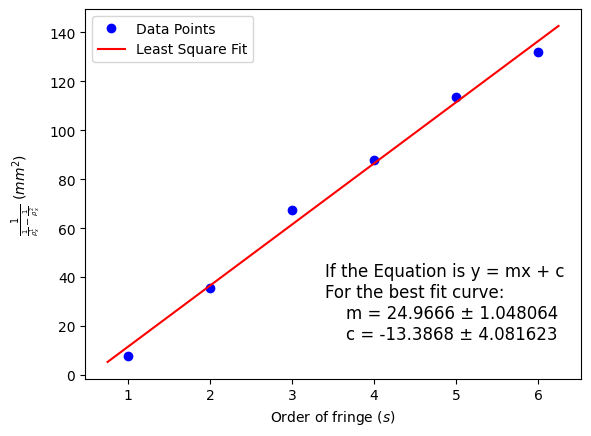
\includegraphics[width=0.8\columnwidth]{images/1.png}
        \caption{$(\frac{1}{\rho_{x}^1}-\frac{1}{\rho_{x}^2})^{-1}$ vs Order of fringe $(s)$}
    \end{figure}

    \begin{figure}[H]
        \centering
        \label{graph:2}
        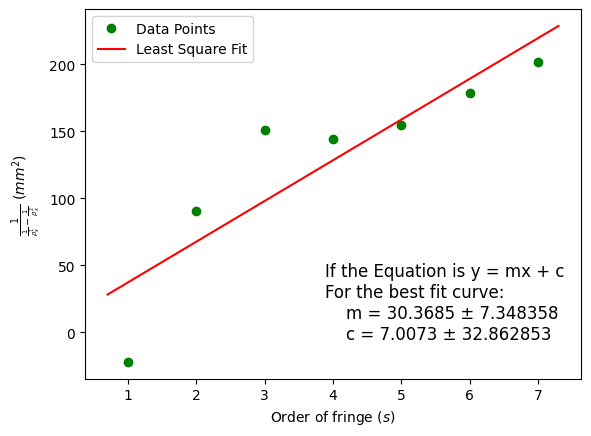
\includegraphics[width=0.8\columnwidth]{images/2.png}
        \caption{$(\frac{1}{\rho_{x}^2}-\frac{1}{\rho_{x}^3})^{-1}$ vs Order of fringe $(s)$}
    \end{figure}

    \begin{figure}[H]
        \centering
        \label{graph:3}
        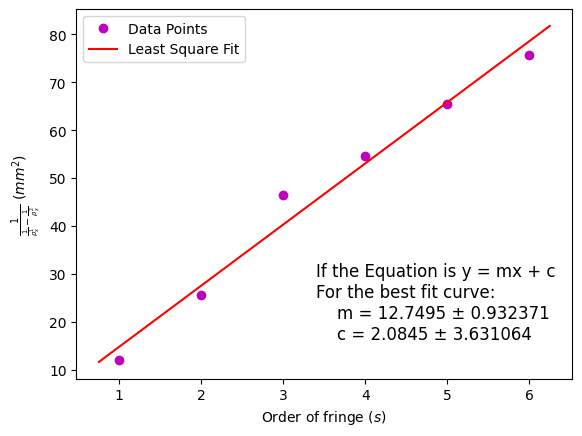
\includegraphics[width=0.8\columnwidth]{images/3.png}
        \caption{$(\frac{1}{\rho_{x}^1}-\frac{1}{\rho_{x}^3})^{-1}$ vs Order of fringe $(s)$}
    \end{figure}

    Using eq. (18),
   \begin{itemize}
       \item For $m_1$ and $m_2$, $Y_{12}$ = 65.48 GPa
       \item For $m_2$ and $m_3$, $Y_{23}$ = 79.65 GPa
       \item For $m_1$ and $m_3$, $Y_{13}$ = 66.88 GPa
   \end{itemize}

   Thus, average value of Y = 70.67 GPa

   \subsubsection{Calculation of Poisson's Ratio ($\sigma$)}

     We can rearrange equation (16) to form 
     \begin{equation}
         \rho_x(s) = \sigma \rho_y(s)
     \end{equation}

      which is of form $y=mx+c$, where $m=$slope and $c=$ y-intercept of a straight line. Thus we can plot this $rho_x(s)$ vs $\rho_y(s)$ to find out $\sigma$ which is equal to the slope ($m$).

      \begin{figure}[H]
        \centering
        \label{graph:4}
        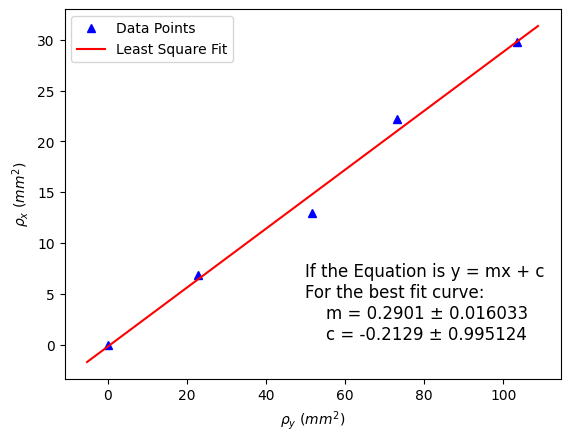
\includegraphics[width=0.8\columnwidth]{images/4.png}
        \caption{$\rho_x$ vs $\rho_y$ for m = 200g}
    \end{figure}

    \begin{figure}[H]
        \centering
        \label{graph:4}
        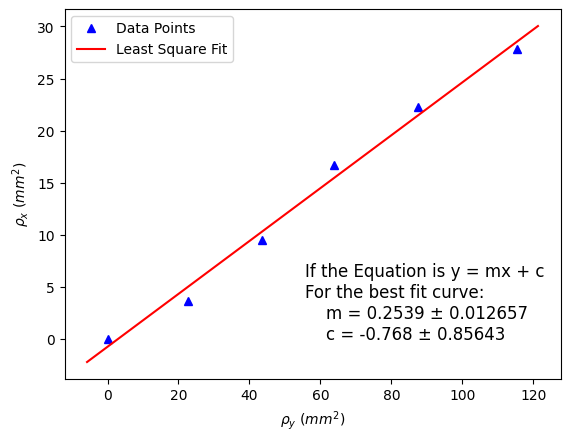
\includegraphics[width=0.8\columnwidth]{images/5.png}
        \caption{$\rho_x$ vs $\rho_y$ for m = 250g}
    \end{figure}

    \begin{figure}[H]
        \centering
        \label{graph:4}
        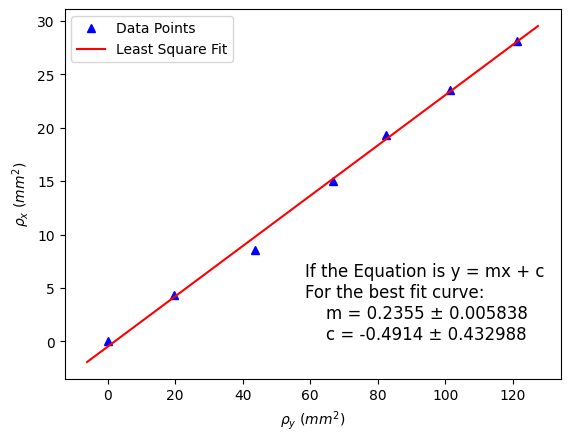
\includegraphics[width=0.8\columnwidth]{images/6.png}
        \caption{$\rho_x$ vs $\rho_y$ for m = 300g}
    \end{figure}

    Thus, the average value of $\sigma$ is observed to be 0.2549.